\section{Taxonomía de Arquitecturas e Implementación}
\label{sec:architecture-taxonomy}

\subsection{Familias de Atención y Mezcladores de Secuencia}
\label{sec:attention-families}

El sistema implementa cuarenta y cuatro mezcladores de secuencia organizados en ocho categorías funcionales que reflejan cómo cada método equilibra expresividad, costo computacional y memoria.
\begin{enumerate}[leftmargin=*]
    \item \textbf{Líneas base densas} (3): atención softmax estándar, atención sigmoide y Grouped-Query Attention (GQA) ofrecen enrutamiento global completo a costo cuadrático.
    \item \textbf{Recurrentes y retentivas} (5): RetNet, Mamba, bloques tipo ODE y Titans mantienen estado para inferencia en tiempo constante mediante recurrencia, espacios de estados selectivos, profundidad continua o memoria en tiempo de prueba.
    \item \textbf{Patrones dispersos} (10): Sparse Transformer, Longformer, SWA con sumideros de atención, BigBird, SparseK, NSA, SpargeAttn, FASA, MSA y SparDA reducen el costo cuadrático mediante dispersión estructurada, selección de tokens o poda sin entrenamiento.
    \item \textbf{Mecanismos con compuerta} (8): GLA, DeltaNet, Gated DeltaNet, Gated DeltaNet-2, HGRN2, FoX, Gated Softmax y KDA introducen control dependiente de los datos sobre retención, olvido y fuerza de actualización.
    \item \textbf{Compresión latente} (10): MLA, GQLA, MLRA, Tucker, IHA, GTA, MTLA, CCA, CCGQA y GMA comprimen el estado clave--valor en cuellos de botella de bajo rango o enrutan mediante una memoria latente de mezcla gaussiana.
    \item \textbf{Memoria condicional} (1): Engram proporciona memoria de lectura/escritura en tiempo de prueba mediante búsquedas aprendidas.
    \item \textbf{Atención de peso rápido} (6): Falcon-1/2/3 y Falcon-1A/2A/3A tratan la transición de estado recurrente como una regla de aprendizaje continuo en línea \citep{zhang_falcon_2026}.
    \item \textbf{Campo geométrico} (1): SSOG aplica un prior geométrico estructurado sobre la matriz de atención \citep{pisoni_ssog_2026}.
\end{enumerate}

\begin{figure}[t]
\centering
\fitfigure{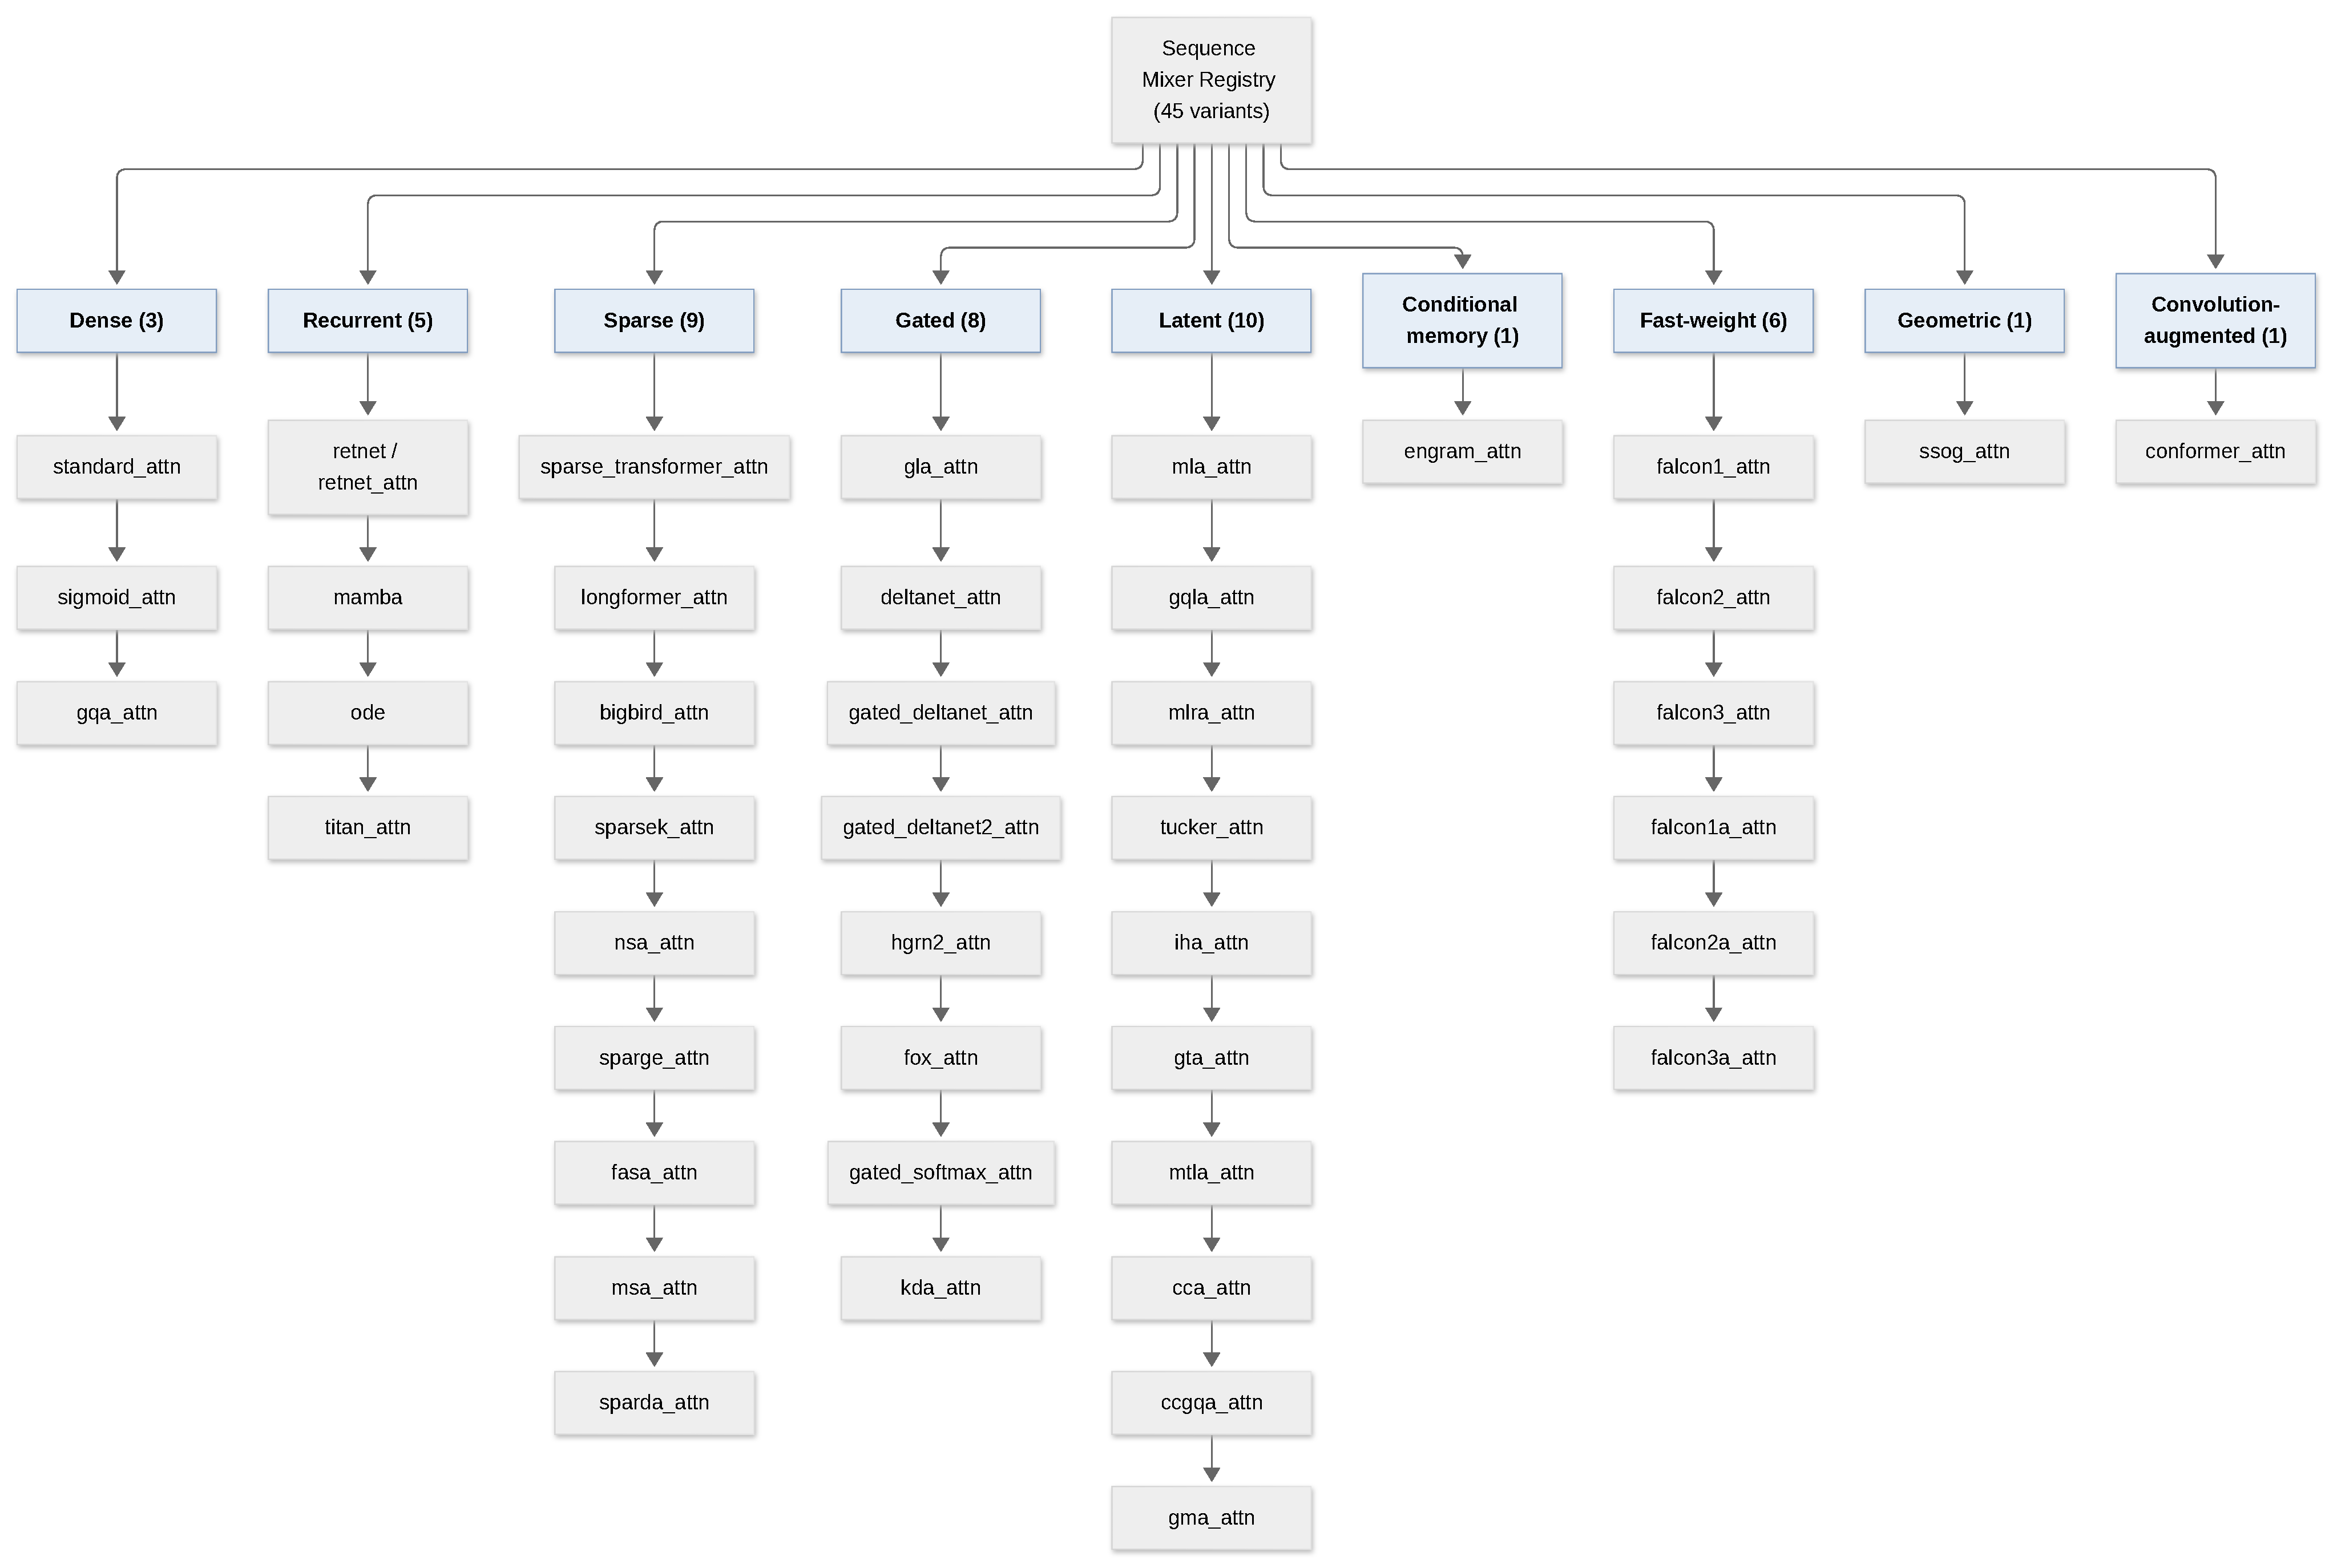
\includegraphics{../paper/figures/mixer-taxonomy.pdf}}
\caption{Taxonomía de los cuarenta y tres mezcladores de secuencia en ocho categorías funcionales. Las líneas base densas ofrecen enrutamiento global completo a costo cuadrático; los métodos recurrentes comprimen el estado para inferencia en tiempo constante; las variantes dispersas restringen el patrón de atención; los mecanismos con compuerta modulan retención y olvido; los métodos latentes comprimen las representaciones clave--valor; la memoria condicional añade búsquedas de lectura/escritura en tiempo de prueba; los métodos de peso rápido formulan la transición de estado como una regla de aprendizaje en línea; los métodos geométricos codifican priors estructurados.}
\label{fig:comprehensive-taxonomy}
\end{figure}

\subsection{Familias Densa y Recurrente}
Las líneas base densas---softmax estándar \citep{vaswani_attention_2017} y atención sigmoide \citep{ramapuram_theory_2024}---y la familia recurrente---RetNet \citep{sun_retentive_2023}, Mamba \citep{gu_mamba_2023}, bloques tipo ODE \citep{zhang_continuous_2021} y Titans \citep{behrouz_titans_2025}---definen el compromiso entre expresividad y eficiencia. Las formulaciones, las formas paralela y recurrente, el pseudocódigo y una tabla comparativa se recopilan en el Apéndice~\ref{sec:annex-transformer}.

\begin{figure}[t]
\centering
\fitfigure{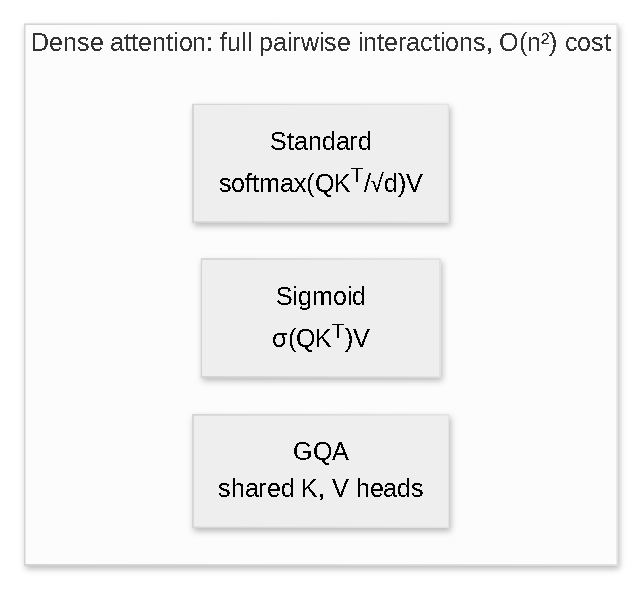
\includegraphics{../paper/figures/dense-map.pdf}}
\caption{Líneas base de atención densa. La atención estándar y la sigmoide calculan interacciones por pares completas; Grouped-Query Attention comparte cabezas clave--valor entre grupos de consultas, reduciendo el tráfico de memoria sin perder la expresividad de la atención completa.}
\label{fig:dense-map}
\end{figure}

\begin{figure}[t]
\centering
\fitfigure{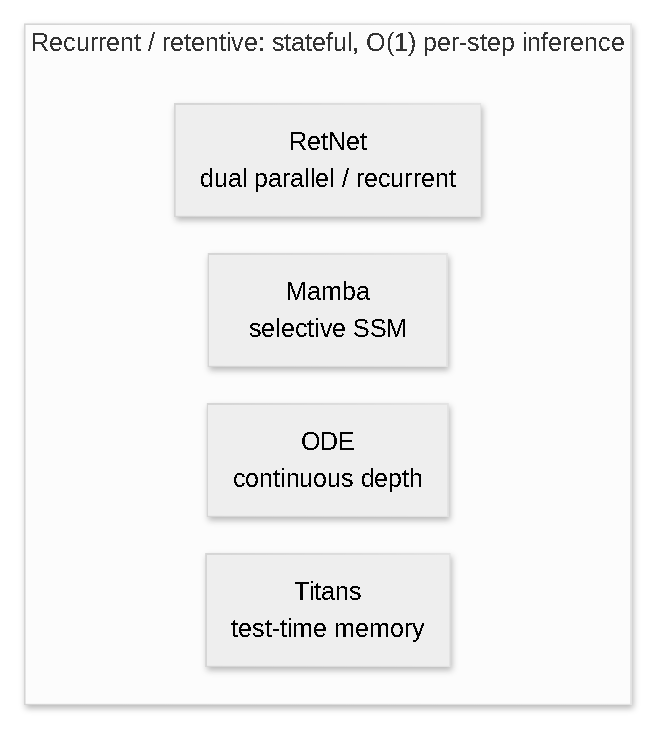
\includegraphics{../paper/figures/recurrent-map.pdf}}
\caption{Familia recurrente y retentiva. RetNet ofrece formas paralela y recurrente, Mamba usa parámetros selectivos de espacio de estados, los bloques ODE modelan profundidad continua y Titans añaden memoria en tiempo de prueba; todos logran inferencia en tiempo constante por paso.}
\label{fig:recurrent-map}
\end{figure}

\subsection{Familia de Atención Latente y de Bajo Rango}
Esta familia comprime el estado clave--valor por token en un latente de bajo rango: MLA, GQLA, MLRA, Tucker, IHA, GTA y MTLA unifican diseños agrupados, latentes, factorizados y temporales. CCA y CCGQA formulan la atención en un latente comprimido con agrupamiento desacoplado, mientras que GMA reemplaza la interacción por pares con enrutamiento probabilístico mediante componentes de mezcla gaussiana aprendidos. Las formulaciones, el pseudocódigo y una tabla comparativa se recopilan en el Apéndice~\ref{sec:annex-latent}.

\begin{figure}[t]
\centering
\fitfigure{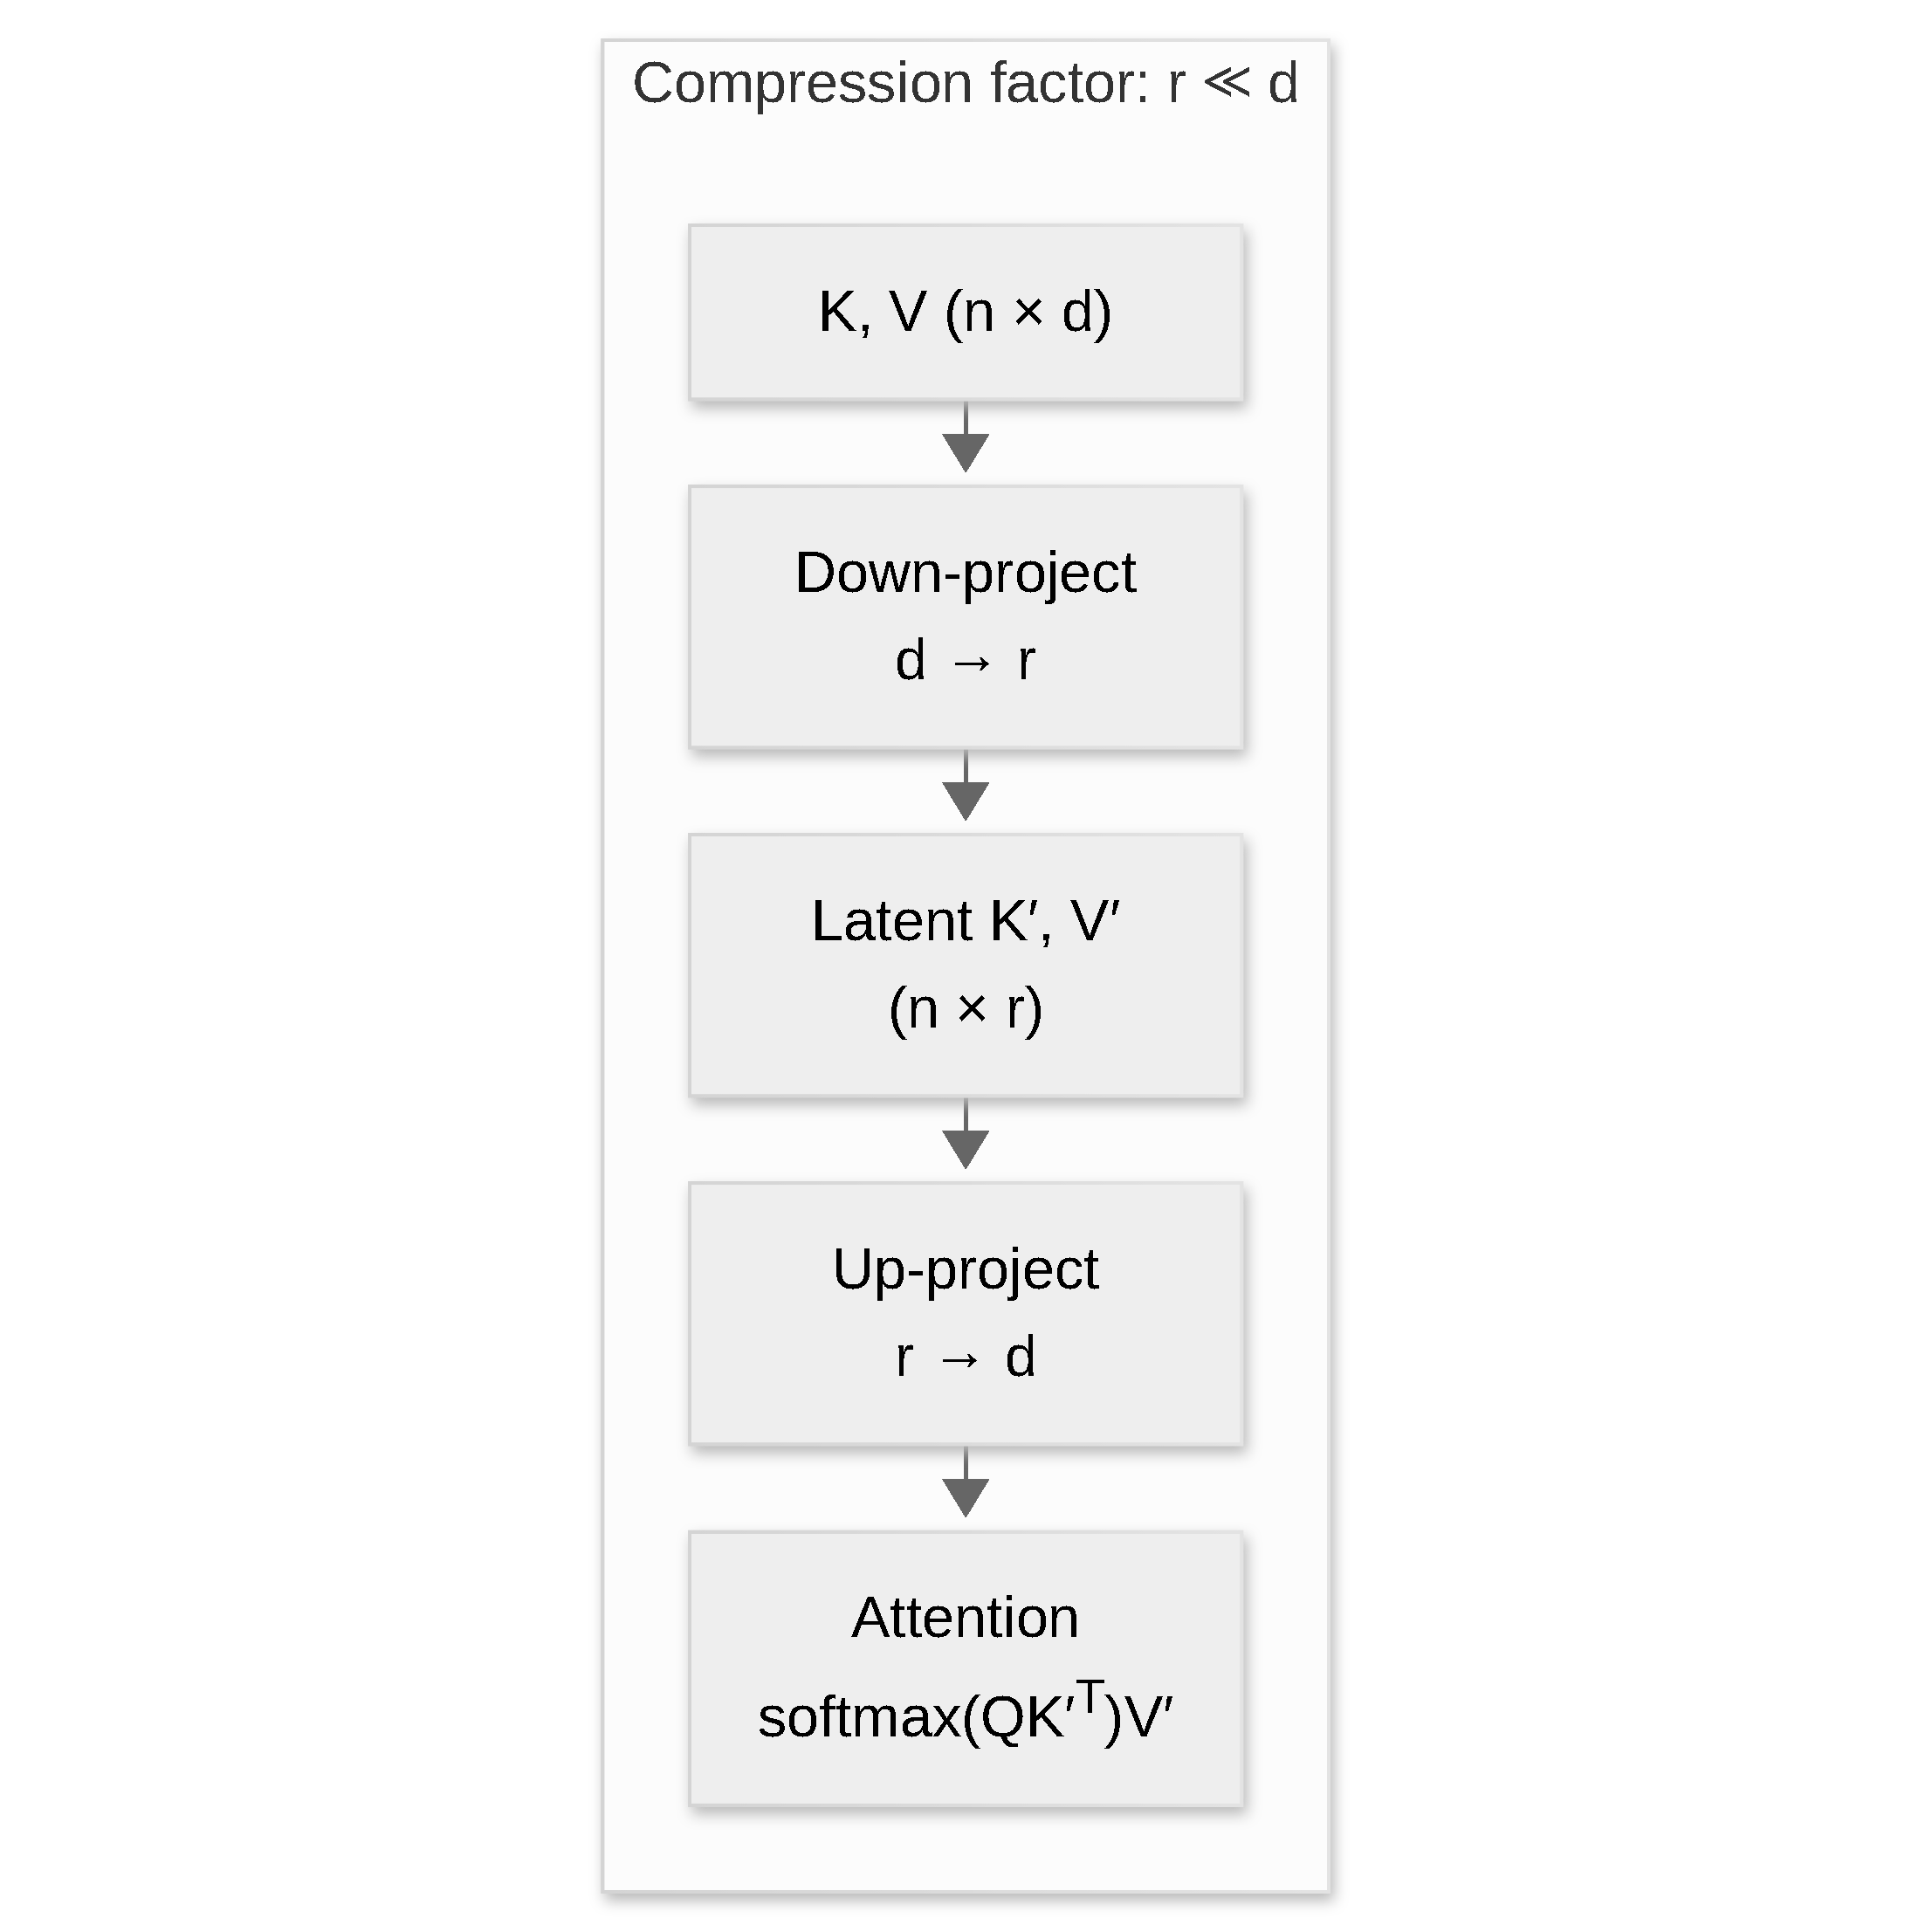
\includegraphics{../paper/figures/latent-map.pdf}}
\caption{Atención latente y de bajo rango. Los pares clave--valor se proyectan a un espacio latente de bajo rango, donde la atención se calcula a menor costo, y se proyectan de vuelta. Las variantes difieren en factorización, intercalado de cabezas, compresión temporal, formulación de covarianza cruzada y enrutamiento probabilístico.}
\label{fig:latent-map}
\end{figure}

\subsection{Extensiones de Atención Dispersa}
El registro incluye diez bloques dispersos \citep{child_sparse_transformer_2019,beltagy_longformer_2020,jolicoeur_sliding_window_2026,zaheer_bigbird_2020,lou_sparsek_2024,yuan_nsa_2025,zhang_spargeattn_2025,wang_fasa_2026,lai_minimax_2026,fu_sparda_2026}. Dos métodos sin entrenamiento, \texttt{fasa\_attn} y \texttt{sparge\_attn}, son solo de evaluación y lanzan un error si se usan durante el entrenamiento; \texttt{swa\_attn} también es sin entrenamiento pero es un mixer entrenable normal, por lo que funciona tanto en entrenamiento como en inferencia. Las formulaciones, el pseudocódigo, las características por bloque y una tabla comparativa se recopilan en el Apéndice~\ref{sec:annex-sparse}.

\begin{figure}[t]
\centering
\fitfigure{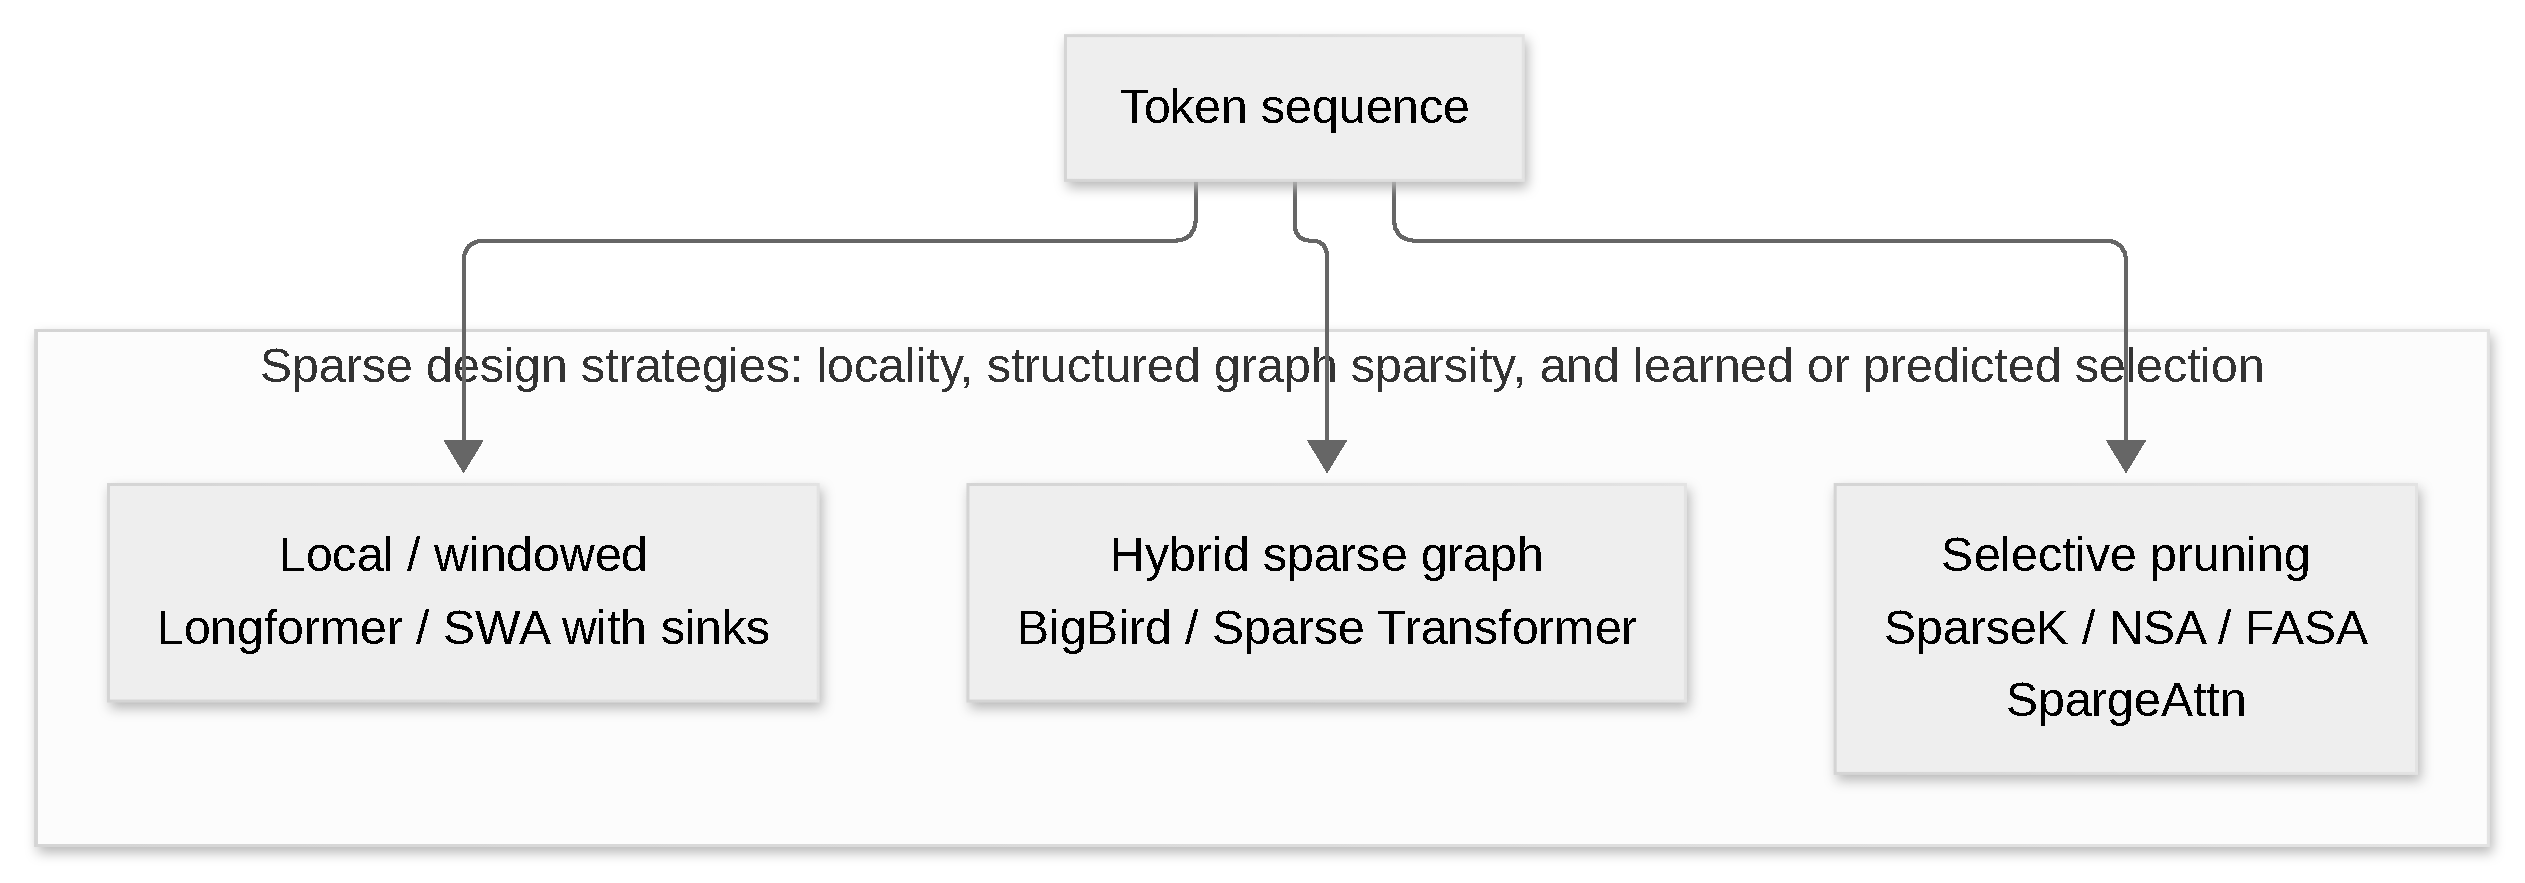
\includegraphics{../paper/figures/sparse-map.pdf}}
\caption{Decisiones de diseño en atención dispersa. Los métodos reducen el costo restringiendo vecindarios, construyendo grafos dispersos o seleccionando solo tokens o bloques de alto valor.}
\label{fig:sparse-map}
\end{figure}

\subsection{Atención con Compuerta y de Peso Rápido}
La familia con compuerta contiene ocho bloques \citep{yang_gla_2023,yang_deltanet_2024,yang_gated_deltanet_2024,hatamizadeh_gated_deltanet2_2026,qin_hgrn2_2024,lin_forgetting_transformer_2025,qiu_gated_attention_2025,kimi_kda_2025}. La compuerta controla qué información sobrevive, ya sea en las actualizaciones de estado recurrente (GLA, variantes de DeltaNet, HGRN2, KDA) o en la ruta de atención completa (FoX, Gated Softmax). Las formulaciones, el pseudocódigo y una tabla comparativa se recopilan en el Apéndice~\ref{sec:annex-gated}.

La atención de peso rápido reformula la actualización recurrente como una regla de aprendizaje continuo en línea; las seis variantes Falcon \citep{zhang_falcon_2026} unifican la regresión estilo DeltaNet y las escrituras de atención lineal bajo semántica de lectura-tras-escritura con tamaños de paso normalizados y olvido explícito. Cada variante incluye un escaneo recurrente de referencia y un kernel paralelo por fragmentos. Las formulaciones, los parámetros de configuración y los resultados publicados se recopilan en el Apéndice~\ref{sec:annex-fast-weight}.

\begin{figure}[t]
\centering
\fitfigure{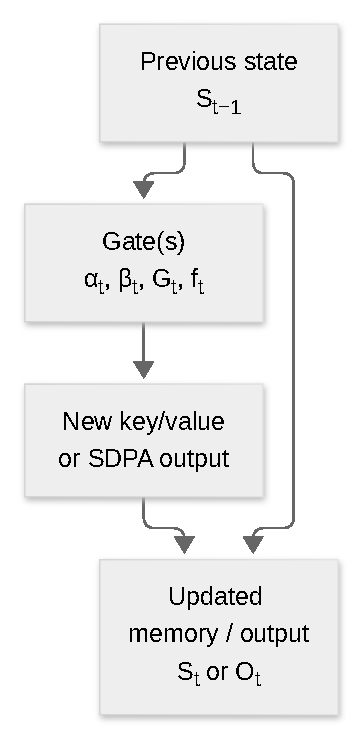
\includegraphics{../paper/figures/gating-template.pdf}}
\caption{Plantilla genérica de compuerta. Una compuerta puede decaer la memoria existente, regular la fuerza de escritura o modular las salidas de atención densa, según la familia de bloques.}
\label{fig:gating-template}
\end{figure}
